\section*{Preamble}
Paper III proposes a spectrally-constrained model for interpreting the total diffuse reflectance spectra obtained with the integrating sphere-based system outlined in Paper~1. The model was developed from the one dimensional diffusion theory approximation of the radiation transport equation\cite{Farrell1992} where each scatter point acts as a point source. The coefficients for the solution to the resulting ordinary differential equation were determined by applying the extrapolated boundary condition.

The necessary corrections to modify a measured reflectance spectrum into the true reflectance spectrum were thoroughly considered. The Single Beam Substitution Error (SBSE) was previously addressed in Paper~1, while the scattering losses that result from calibration with a highly scattering Spectralon\textregistered~standard were investigated in this paper. To determine the functional form of this correction factor (SLCF), mono Monte Carlo simulations were performed and then confirmed with tissue-simulating liquid phantoms.

The order in which these corrections are applied in the fitting algorithm was determined based on the required parameters for each step. The robustness of the model was then tested for effects of noise, and changes in the scattering and background absorption coefficients. Finally, the model was used to interpret the previously collected lidocaine \& epinephrine data from Paper~2 and compared to the Dawson erythema index.\cite{Dawson1980}

All of the work undertaken for this paper was performed by the author of this thesis (further known as ``the author'') under the supervision of Drs. T. Farrell and J. Hayward with the following exceptions; As previously mentioned, the epinephrine study was jointly undertaken by the author and Dr. D. McKee, the liquid phantoms were prepared by Mr. D. Gallino, the spatially-resolved diffuse reflectance measurements were collected and analyzed with the help of Mr. D. Cappon, and the Monte Carlo simulation code was written with significant help by Dr. G. Devenyi. The manuscript was written by the author and edited by Drs. Farrell and Hayward. The manuscript has been altered from its original form to match the style of this thesis.

\section*{Contents}

\begin{center}
	
	\textbf{Modeling changes in the hemoglobin concentration of skin with total diffuse reflectance spectroscopy}
	
	Diana L. Glennie, Joseph E. Hayward, and Thomas J. Farrell
	
	\textit{Department of Medical Physics and Applied Radiation Sciences, McMaster University, 1280 Main Street West, Hamilton, Ontario, L8S 1A8}

	\textit{AND}

	\textit{Department of Medical Physics, Juravinski Cancer Centre, 699 Concession Street, Hamilton, Ontario, L8V 5C2}

\end{center}

\noindent Submitted to the \textit{Journal of Biomedical Optics} on September 25, 2014.

\section*{Abstract}
The ability to monitor changes in the concentration of hemoglobin in the blood of the skin in real time is a key component to personalized patient care. Since hemoglobin has a unique absorption spectrum in the visible light range, diffuse reflectance spectroscopy is the most common approach. Although the collection of the diffuse reflectance spectrum with an integrating sphere has several calibration challenges, this collection method is sufficiently user-friendly that it may be worth overcoming the initial difficulty. Once the spectrum is obtained, it is commonly interpreted with a log-inverse-reflectance (LIR) or ``absorbance'' analysis that can only accurately monitor changes in the hemoglobin concentration when there are no changes to the non-hemoglobin chromophore concentrations. This paper addresses the difficulties associated with collection of the diffuse reflectance spectrum with an integrating sphere and proposes a model capable of retrieving relative changes in hemoglobin concentration from the visible light spectrum. The model is capable of accounting for concentration changes in the non-hemoglobin chromophores and is first characterized with theoretical spectra and liquid phantoms. The model is then used in comparison with an LIR analysis on temporal measurements from blanched and reddened human skin.

\section{Introduction}
The knowledge of changes in blood volume in tissue is a valuable asset when monitoring the effects of a wide range of therapeutic interventions, from radiation therapy\cite{Farrell2004,Fitzgerald2008,Russell1994,Wengstrom2004} to skin-flap transplants.\cite{Steele2011} The most common method of monitoring changes in skin perfusion or blanching is by visual inspection.\cite{Wengstrom2004, CTCAE403} While widely accessible, this approach is subjective and is prone to inter- and intra- observer error.\cite{Diffey1991} Monitoring changes in skin perfusion to gauge patient progress would be more reliable if an objective, quantitative approach were available.

Steady-state diffuse reflectance spectroscopy (DRS) measures the wavelength-dependent intensity of light that has entered and scattered back out from a sample.\cite{Kim2011} Since the amount of reflected light is dependent on the absorption coefficient $\mu_a$, which is itself a function of the individual chromophore concentrations (such as oxy- and deoxy-hemoglobin, and melanin), it is a good candidate for the task. There are several different approaches and technologies available for obtaining a diffuse reflectance spectrum, each with their own set of advantages and disadvantages.

\subsection{Measurement of Diffuse Reflectance Spectra}
Spatially-resolved diffuse reflectance (SRDR) is one of the most common approaches for determining optical properties from reflectance spectra. Typically, fiber optics are placed at increasing radial distances from a source fiber and the measured intensities can be used to determine both the absorption and reduced scattering coefficients.\cite{Kim2011} However, SRDR is rarely used in the clinical setting due to the many difficulties associated with its implementation. SRDR returns most accurate results when there is good coupling between the fiber optics and the measurement surface. Also, the results may be sensitive to local inhomogeneities, such as freckles, hair, and localized vasculature that may alter the individual fiber measurements. Since the signal drops off rapidly with distance, a high quality spectrometer is required to span the required dynamic range and establish the rate of decrease in intensity as a function of radial distance, making it expensive and difficult to calibrate.

An alternative is to use a single fiber-optic source-collector pair geometry. This has many of the same complications as the spatially-resolved approach except it is not as expensive and is much easier to calibrate. It is still error prone if tissue contact is compromised or if there is a local inhomogeneity, but the source/detector geometry can be selected to match a specific range of expected optical properties and minimize the effect of high scattering.

Another measurement technique is an integrating sphere (IS) based system.\cite{Marchesini1991,Zhang2012} In these systems, the total light diffusely reflected by a single integrating sphere from a sample is compared with that collected from a highly reflective calibration plate. Such systems do not have any of the difficulties associated with fiber-based geometries. They are inexpensive, easy to ensure sample coupling, and are insensitive to pathlength considerations and local inhomogeneities since they measure the average reflectance over an area. However, this approach has its own set of challenges that must be addressed before an accurate reflectance spectrum can be obtained. Once they have been overcome, this method is easily implemented and has a low assembly cost.

\subsection{Analysis of a Diffuse Reflectance Spectrum}
The absorption spectrum for a purely absorbing (no scattering) solution can be determined with the Beer-Lambert law by measuring the light transmitted through a sample in a cuvette with a spectrophotometer.\cite{Niemz2007} Since the pathlength is fixed, the transmission measurement is often expressed as the common logarithm of the ratio of the incident intensity to the transmitted intensity, known as the ``absorbance''. This approach has been adopted in tissue optics to analyze a diffuse reflectance spectrum by calculating the common logarithm of the reciprocal (inverse) of the reflectance spectrum (known as “LIR”).\cite{Dawson1980,Feather1989} However, \emph{in vivo}, only the reflected light intensity as opposed to the transmitted light intensity can be measured due to the different geometry. Also, since the tissue is highly scattering, the pathlength is no longer fixed and known. This is accounted for by introducing a pathlength correction factor $l(\lambda)$ into the LIR term. Since this factor is wavelength-dependent and unknown, only changes in chromophore concentrations are possible with this approach. The change in LIR (including the unknown pathlength correction factor) is equated directly to the absorption from the individual chromophores, which is expressed as the products of the concentrations $c_i$, and extinction coefficients $\varepsilon_i(\lambda)$,\cite{Kollias2010}

\begin{equation}
	\begin{split}
			\Delta LIR(\lambda)/l(\lambda)  & = \Delta c_{HbO}(\lambda)\varepsilon_{HbO}(\lambda)  + \Delta c_{Hb}(\lambda)\varepsilon_{Hb}(\lambda) + \Delta c_{mel}(\lambda)\varepsilon_{mel}(\lambda) \\
			& + \Delta c_{H_2O}(\lambda)\varepsilon_{H_2O}(\lambda) + \Delta c_{scat}(\lambda)\varepsilon_{scat}(\lambda)
	\end{split}
\end{equation}

It is common to use the LIR values at wavelengths above 650 nm to approximate the contribution from the non-hemoglobin chromophores, and to use the LIR value at 550 nm to approximate the contribution from scatter.\cite{Hajizadeh-Saffar1990} This approach is intended to remove all but the hemoglobin terms and has been shown to successfully approximate changes in skin perfusion, but only in the instance where there are no changes in the non-hemoglobin chromophore concentrations or scattering conditions. Otherwise, the correction method fails and the recovered hemoglobin concentrations are no longer linear with respect to actual changes to the LIR spectrum.

Depending on the duration over which the measurements are performed, it may be reasonable to assume that there are no changes to the melanin and background absorption components or to the reduced scattering coefficient. However, if these values have changed, a robust model should have the ability to account for them. A spectrally-constrained theoretical approach relies on known absorption and scattering coefficient spectra to model the diffuse reflectance spectrum. Since there exists a large body of data on the extinction coefficients for the major constituents of human skin in the visible-to-near-infrared region, this approach may be an ideal solution. In this manuscript, such a model will be applied to total diffuse reflectance spectra obtained with an inexpensive IS-based DRS measurement system. Next, deviations to the model introduced by the use of an IS will be identified and addressed. Finally, the fully-characterized system and model will be used in an in vivo study in which the results will be compared to a common LIR analysis.

\section{Theory}
An appropriate model is required to interpret the total diffuse reflectance spectra obtained from an IS. For a sufficiently large illumination port geometry, the incident light on the skin can be accurately approximated by a broad beam light source perpendicularly incident on a semi-infinite, homogeneous medium. However, for realistic IS sizes, there are a number of factors that introduce deviations from the simple model that will require corrections. While it may be standard procedure to apply all of the corrections to the calculated spectrum, the available information mandates that some of the corrections be applied to the collected spectrum. Therefore, special consideration is required during the development of a fitting algorithm.

\subsection{Forward Model Derivation}
\label{sec:forward_model}
There are several different ways of modeling light transport in tissue. One such approach is the Boltzmann Radiative Transport Equation (RTE), which describes the stochastic behavior of neutral particles such as photons.\cite{Duderstadt1976} When sufficiently far from a boundary within a turbid material, the RTE can be accurately approximated by the steady-state diffusion equation,\cite{Farrell1992}

\begin{equation}
\label{eq:SSDE}
	\nabla^2\Psi(r) - \frac{\mu_a}{D}\Psi(r) = S(r).
\end{equation}

The light fluence rate $\Psi(r)$, is dependent only on the absorption coefficient $\mu_a$, the reduced scattering coefficient $\mu_s'$, and the source term $S(r)$. The sum of absorption and reduced scattering coefficients is the reduced total interaction coefficient $\mu_t'$. The source term, that represents photons scattered out of the primary beam, is typically approximated by an isotropic spherical harmonic term $-S_0(r)/D$, where $S_0(r)$ decays with depth and $D$ is the diffusion constant,

\begin{equation}
	D = \frac{1}{3\mu_t'}.
\end{equation}

For a normally incident, semi-infinite broad beam light source, Equation~\ref{eq:SSDE} collapses into one dimension,

\begin{equation}
\label{eq:ss_1d}
	\frac{d^2\Psi(z)}{dz^2} - \mu_{eff}^2\Psi(z) = -\frac{\mu_s'}{D}I_0e^{-\mu_t'z},
\end{equation}

where

\begin{equation}
\mu_{eff}^2 \equiv \frac{\mu_a}{D}.
\end{equation}

This equation has a closed form solution that can be determined by considering the boundary conditions.\cite{Farrell1992}

By applying the definition that total diffuse reflectance is the fraction of the incident photon current exiting the tissue surface to the solution to Equation~\ref{eq:ss_1d}, an equation for the wavelength-dependent diffuse reflectance is produced,

\begin{equation}
\label{eq:diff_refl}
	R_d = \frac{\mu_s'}{\left[\mu_t' + \mu_{eff}\right]\left[1 + 2AD\mu_{eff}\right]}.
\end{equation}

\subsection{Integrating Sphere Effects on Reflectance Measurements}
When the total diffuse reflectance spectrum is collected with an IS, the finite geometry violates some of the assumptions made in Section~\ref{sec:forward_model} regarding the broad beam geometry. Corrections can be applied to account for these deviations from the theoretical model, thereby restoring some of its accuracy. There are three major violations which must be addressed: (1) the specular reflectance, (2) the single-beam substitution error, and (3) the scattering losses.

Specularly reflected light has not penetrated the tissue of interest and, therefore, carries no information about the tissue optical properties. The amount of light that penetrates the tissue or is specularly reflected depends on the index of refraction of the material and is on the order of four percent for human tissue.\cite{Welch2011} If the specularly reflected light were to be collected in addition to the diffusely reflected light, it could account for a significant portion of the total detected signal (depending on the skin type) which would yield inaccurate results. To reduce the contribution from specularly reflected light, an illumination geometry should be chosen such that none of the specularly reflected light can enter the detection fiber. In this way, only light that has penetrated, and been remitted from, the tissue will be detected. This can also be achieved through the implementation of a baffle; however it is not generally preferred as it disrupts the internal surface of the sphere, leading to substantial non-uniformities in smaller spheres.\cite{Labspherea}

Single-beam substitution error (SBSE) is due to the normalization procedure that converts a single intensity measurement $s_m$, into reflectance by subtracting the background signal $s_{bg}$, and comparing it to the signal from a highly reflective calibration standard $s_{cal}$,\cite{Springsteen1998}

\begin{equation}
	R_m = \frac{s_m - s_{bg}}{s_{cal} - s_{bg}}.
\end{equation}

When the calibration standard is replaced with the sample to be measured, there is a decrease in the total flux within the sphere due to the considerably higher absorption in the sample as well as multiple scattering, which leads to a lower reflectance. Therefore, a correction factor for SBSE would be both sphere and reflection dependent, and can be determined empirically with a set of diffuse reflectance standards.\cite{Labspherec,Glennie2014b}

The final IS effect to be accounted for is the decrease in detected signal due to the finite port size. Near the edge of the detection port, there is an annular region where the light that enters the sample will migrate away from the detection port, resulting in a small decrease in the reflected signal. For the calibration standard, which has a significantly higher scattering coefficient compared with human tissue,\cite{Tseng2008} this region (and the deviation from the model) is small. However, as the reduced scattering coefficient decreases, the pathlength increases and the region and its influence increases. This phenomenon, similar to that investigated by Zhu \emph{et al.},\cite{Zhu2014} can be accounted for with a scattering losses correction factor (SLCF) that is a function of both the absorption and reduced scattering coefficients, and can be determined empirically or with Monte Carlo (MC) methods.

\subsection{The Fitting Algorithm}
\label{sec:fitting_algorithm}
In the absence of any IS effects, the calculated broad beam diffuse reflectance model would simply be fit to the measured reflectance spectrum using the concentrations of absorbers as parameters in a spectrally-constrained least-squares approach. The concentrations of the major chromophores $c_i$, would be the fitting parameters multiplied with their corresponding extinction coefficient spectra $\varepsilon_i(\lambda)$, to produce the absorption coefficient spectrum,

\begin{equation}
\mu_a(\lambda) = \sum_i c_i \times \varepsilon_i(\lambda).
\end{equation}

In the visible light spectrum, the three major chromophores that contribute to the absorption coefficient are oxy-hemoglobin, deoxy-hemoglobin, and melanin. Each has a well-established extinction coefficient spectrum as shown in Figure~ 1.\cite{Prahl2001} While both eumelanin (black/brown) and pheomelanin (yellow/red) are found in human skin, eumelanin is the dominant form, therefore its spectrum was selected for use in the fitting algorithm. Additional chromophores such as bilirubin and water do not contribute significantly in this region, however a fourth term can be included to account for the base absorption by all other minor chromophores in the skin layers. The shape of this component is exponential with respect to wavelength, according to the Huang and Jacques data from bloodless rat skin,\cite{Jacques1998}

\begin{equation}
	\mu_{a~base} = a \times \exp \left[\frac{-(\lambda - 154)}{66.2}\right] + b~~\left[mm^{-1}\right]
\end{equation}

where $a$ and $b$ are scaling (fitting) parameters.

\begin{figure}
	\centering 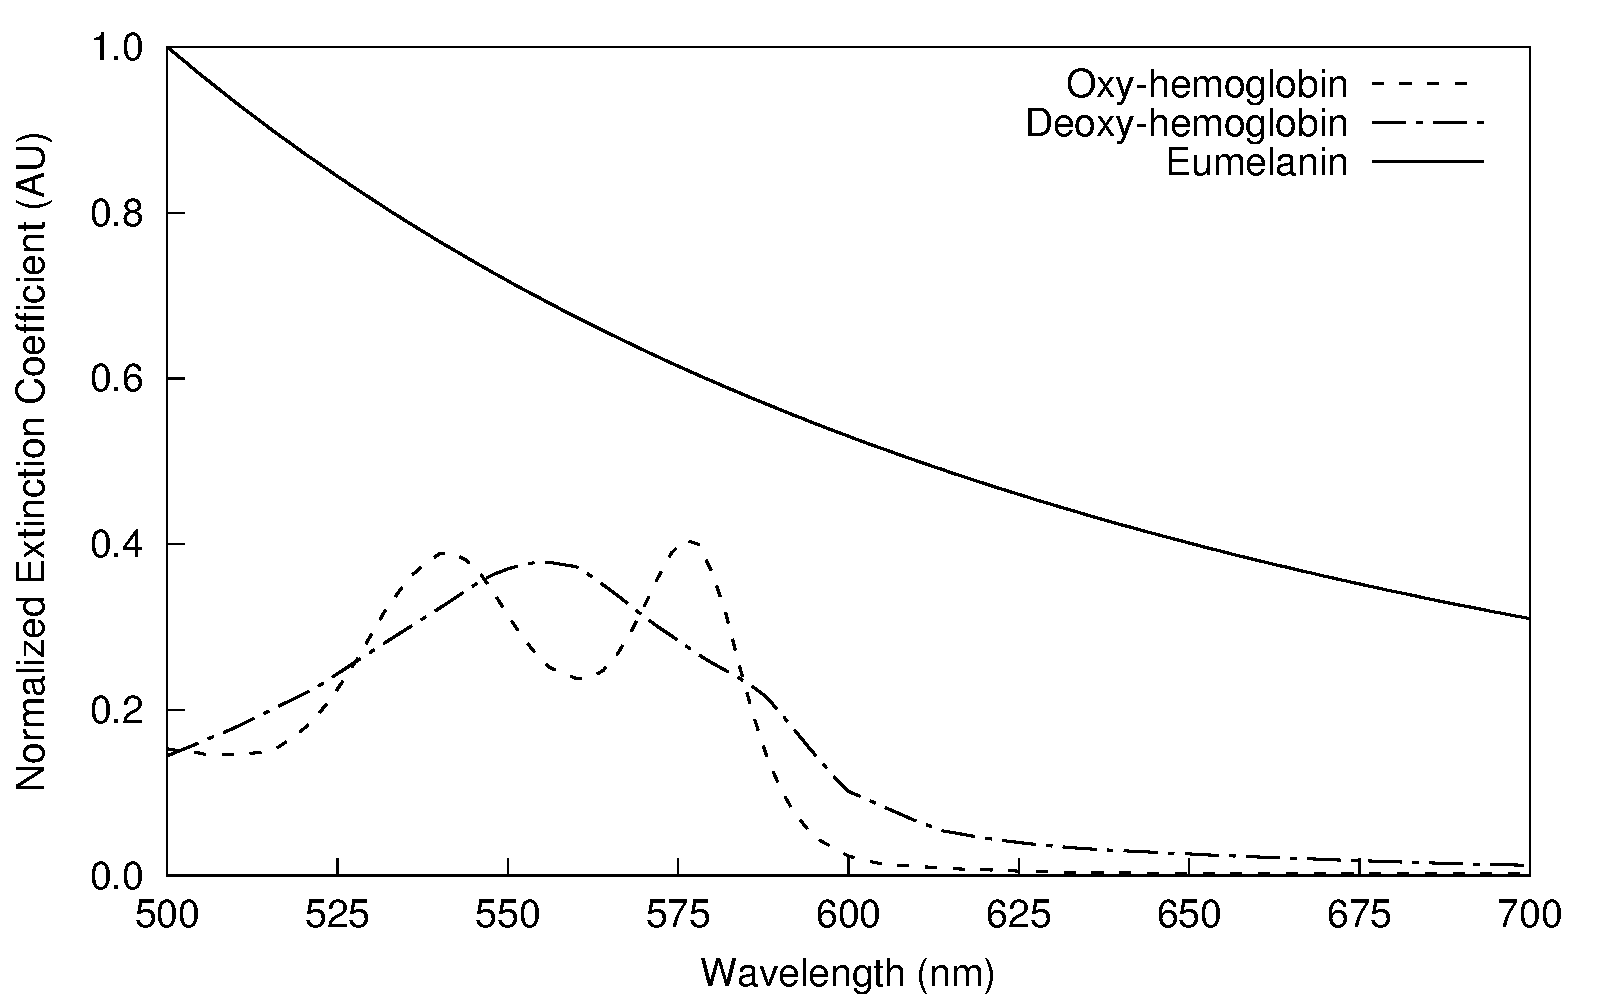
\includegraphics[width=0.8\textwidth]{figures/p3-chromophores.png}
	\caption[Major chromophore extinction coefficient spectra]{\label{fig:p3-chromophores}Normalized extinction coefficient spectra for the three major chromophores found in human skin.}
\end{figure}

This baseline absorption spectrum has a similar broad-spectral shape to the melanin extinction coefficient spectrum. Therefore, it will be impossible to separate the contributions from these two concentrations. Since the goal of this study is to monitor changes in hemoglobin concentration, these two absorption components were combined following fitting and considered together as a single background absorption term. The final absorption term consisted of five components with five fitting parameters.

With only a single measurement (that of the total diffuse reflectance), the contributions from absorption and scattering are not separable. Therefore, an assumption of the reduced scatter spectrum is necessary to extract information on the absorption coefficient spectrum. This approach was deemed valid since there is only a small amount of variation in scatter between individuals for a particular tissue type.\cite{Kim2011} The chosen spectrum should closely approximate scatter in both the epidermis and dermis since the skin is being modeled as a homogeneous slab of tissue. Due to the protein structure of these two layers (e.g keratin, collagen fibers), the reduced scattering spectrum for visible light has both Rayleigh and Mie scattering contributions and can be determined as the sum of these two components,\cite{Jacques1998}

\begin{equation}
	\mu_{s~Mie}'(\lambda) = 2 \times 10^4 \lambda^{-1.5}~~[mm^{-1}]
\end{equation}

\begin{equation}
	\mu_{s~Rayleigh}'(\lambda) = 2 \times 10^{11}\lambda^{-4}~~[mm^{-1}]
\end{equation}

The resultant absorption and reduced scattering coefficient spectra would then be used to calculate the spectral broad beam reflectance, according to Equation~\ref{eq:diff_refl}. The correct concentrations would be those parameters that minimize the sum-of-squares.

However, as previously stated, the effects of the IS must be accounted for and the model should be adjusted accordingly. Ideally, all corrections would be made to the measured reflectance spectrum to reproduce the broad beam reflectance spectrum being modeled in the calculated spectrum. Since the SLCF is a function of the absorption and scattering coefficients, it was easier to apply the SLCF to the calculated reflectance spectrum where the input optical properties are known.

In addition to the IS effects, the fitting algorithm must account for the spectral resolution of the spectrometer. Depending on the full-width-at-half-max (FWHM) of the spectral response function, it may be necessary to de-convolve the measured reflectance spectrum with the chosen response function. However, since deconvolutions are prone to noise amplification and signal stability issues, they are not preferred.\cite{Kundur1996,Gonzalez2003} Instead, the calculated reflectance spectrum was convolved with the instrument response function and compared with the measured spectrum. A flow chart for the fitting algorithm is shown in Figure~\ref{fig:p3-flowchart}.

\begin{figure}
	\centering 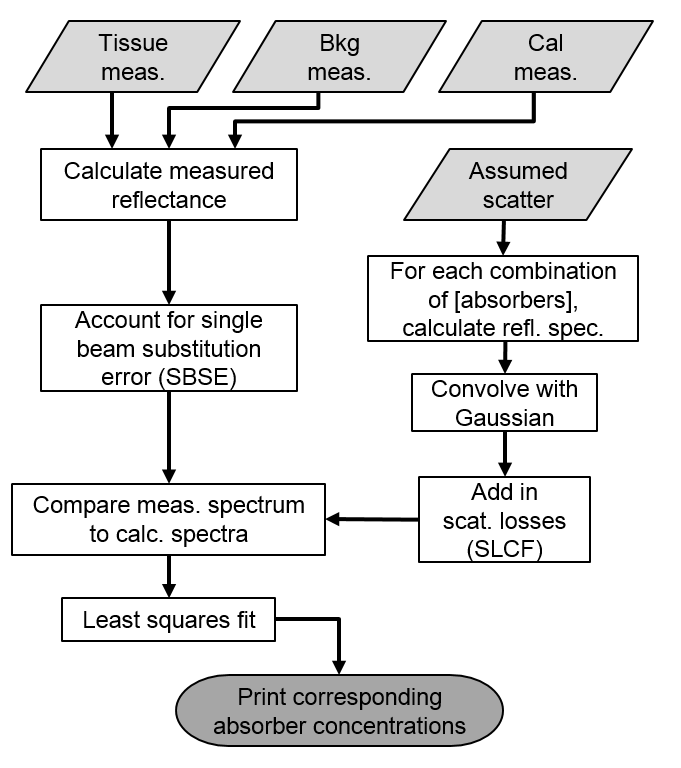
\includegraphics[width=0.6\textwidth]{figures/p3-flowchart.png}
	\caption[Fitting algorithm flow chart]{\label{fig:p3-flowchart}A flow chart describing the fitting algorithm to be applied to total diffuse reflectance measurements. The single beam substitution error is applied to the measured spectrum while all other corrections are applied to the calculated spectrum.}
\end{figure}

\section{Methods \& Materials}
The robustness of the model was tested using reflectance spectra representing a variety of tissue optics situations. Following the characterization of the model, the SBSE correction factor and the SLCF were determined. The SBSE correction factors were established following an accepted empirical approach.\cite{Labspherec} Since there was no established method for accurately assessing and correcting for the scattering losses, one was developed using Monte Carlo simulations and tissue-simulating phantoms. Following a complete characterization of the model, it was used in an in vivo study to extract blood concentrations in human skin from diffuse reflectance spectra obtained with an IS.

The IS-based system used to collect total diffuse reflectance spectra throughout this paper has been described previously.\cite{Glennie2014b} Briefly, the system consists of a tungsten halogen light source coupled via optical fibers to an IS (manufactured in-house) and a computer-based spectrometer. The collection fiber directly illuminates the grating of the spectrometer, acting in place of a slit. The spectral resolution of the system, measured using a mercury-argon calibration source, is 10 nm FWHM. The spectrometer range was 340-997 nm, encompassing 2048 discrete wavelengths. Since the chromophores of interest do not have significant spectral features below 500 nm or above 700 nm, the measurement spectra were analyzed only within this wavelength range. The typical measurement uncertainty did not exceed two percent across this interval for true reflectance values above 20 percent.

\subsection{Characterization of the Model}
In order to investigate the robustness of the model, sample spectra were generated using the forward model described in Section~\ref{sec:forward_model} which were then convolved with the IS system spectral response (represented by a Gaussian function). Two melanin concentrations were selected to yield Type III and Type V representative skin types on the Fitzpatrick scale.\cite{Fitzpatrick1988} For each melanin concentration, three hemoglobin concentrations were chosen, corresponding to blanched, normal, and reddened skin respectively, for a total of six representative baseline diffuse reflectance spectra. When these unmodified spectra were fitted with the model, the hemoglobin concentrations were recovered to within 0.2 percent of the input values. These spectra were then used to determine the effect of noise on the model's performance as well as the impact of an incorrect reduced scattering coefficient spectra or of a change in the background absorption spectrum.

\subsubsection{Testing the Effect of Noise}
To test the effect of noise in the signal on the model performance, Gaussian random noise ranging from one to ten percent was added to each of the six sample spectra. This process was repeated five times for each baseline spectrum in order to perform a statistical analysis on the results. The noisy spectra were then fitted with the model and the hemoglobin concentrations were recovered. The mean and standard deviation of the difference between the recovered concentration and the input concentrations for oxy- and deoxy-hemoglobin were determined for each noise level.

\subsubsection{Testing the Effect of an Incorrect Scatter Coefficient Spectrum}
Since the scattering properties of human epidermis and dermis do not vary widely between individuals, the model incorporates a constant average reduced scattering coefficient spectrum. While it is probable that it does not accurately represent the scattering for a given individual, the deviation from this chosen spectrum is expected to be small. To investigate the possible effect of these differences, eight Fitzpatrick Type III reflectance spectra were produced with decreasing and increasing amounts of total hemoglobin concentrations from 25 to 200 percent of a baseline amount (oxygen saturation of 84 percent)\cite{Arimoto2006} and with two percent noise. Each spectrum was fit using a different assumed, reduced scattering coefficient spectrum, from 25 to 200 percent of the original, input reduced scattering spectrum. The differences between the recovered total hemoglobin concentration and the input concentration were calculated.

\subsubsection{Testing the Effect of Changes in Background Absorption}
As mentioned in Section~,\ref{sec:fitting_algorithm} absorption by melanin and the structural components in skin were combined into a single background absorption term. Depending on the timeline over which measurements are taken, it is possible that the contributing absorber concentrations may change. The model is expected to correctly account for this change and to accurately recover the hemoglobin concentrations. To verify this expectation, a set of Fitzpatrick Type III spectra were produced with simultaneously increasing hemoglobin (up to 200 percent) and background absorbers (up to 40 percent). If the increase in background absorption was due solely to the increase in melanin concentration, a 40 percent increase would correspond to a reclassification of a Type III skin type into a Type IV skin type, which is highly improbable but would be visibly noticeable and so represents the upper limit of absorption increase. These spectra were fitted and the hemoglobin concentrations were recovered and compared to the input values.

\subsection{Determination of the Scattering Losses Correction Factor}
\label{sec:SLCF_methods}
The magnitude of the scattering losses is sphere dependent and inversely proportional to the absorption and reduced scattering coefficients, i.e., for a given IS geometry, it will increase as either the absorption or scattering coefficients decrease. Monte Carlo (MC) simulations were used to determine the functional form of the SLCF and empirical measurements were used to verify and obtain the exact parameters of the functional form.
A variation of the standard MC simulation called a Mono MC\cite{Kienle1996a} (or “White MC”)\cite{Alerstam2013} was used to economize the computationally expensive simulation. Under this approach, photons were tracked through the material with only scattering properties defined, and the effect of absorption was applied afterward. The MC geometry matched the actual IS measurements, with a sphere wall reflectance coefficient of 0.95. The semi-infinite homogeneous tissue was assigned a refractive index of 1.33 and an anisotropy factor of 0.9.\cite{Wang1995} Simulations were performed for a range of reduced scattering coefficients from 0.50 to 4.00 $mm^{-1}$. For each simulation, a range of absorption coefficients from 0.01 to 10.00 $mm^{-1}$ was applied to obtain simulated reflectance values $R_{sim}$, which represented the reflectance measured with the IS. These values were then combined with reflectance values calculated with the model $R_{calc}$, to achieve SLCFs as follows,

\begin{equation}
	SLCF\left(\mu_a, \mu_s'\right) = \frac{R_{sim}}{R_{calc}}.
\end{equation}

Once the functional form was determined, twenty liquid phantoms were measured with the IS to confirm the fit. These phantoms included different concentrations of commercially available green food coloring and Intralipid\textregistered (Baxter, Toronto, Ontario) such that the absorption ranged from 0.01 to 0.38 $mm^{-1}$ and the reduced scattering coefficient ranged from 0.45 to 3.5 $mm^{-1}$. Both extinction coefficient spectra were determined with a spatially-resolved diffuse reflectance spectrometer while that of the green food coloring was additionally characterized with a UV/Visible Spectrophotometer (Varian Cary 50 Bio, Cary, NC).

The phantoms were measured with the IS system as well as with the spatially-resolved system. The SBSE was applied to the measured reflectance, and the concentrations extracted from the spatially-resolved system were used to calculate the diffuse reflectance with the model which was then convolved with the spectral response function. The ratios of these two sets (representing the SLCF), combined with the absorption and reduced scattering coefficients created a set of triplets which was fitted using the previously obtained function form for the SLCF.

\subsection{\emph{In Vivo} Study}
An \emph{in vivo} experiment was performed to determine the time to maximal vasoconstriction following the injection of epinephrine. Volunteers were made to lay quietly on a bed for ten minutes, during which time five baseline measurements were performed. They were then injected subcutaneously in both upper arms with either 5 cc of 1 percent lidocaine (plain) or 5 cc of 1 percent lidocaine with 1:100,000 epinephrine (0.01 mg/mL) (AstraZeneca Canada, Inc., Mississauga, Ontario) in order to induce perfusion or blanching, respectively. Reflectance spectra were obtained with the IS system every minute for 30 minutes and then every two minutes for another 90 minutes. The spectra were processed using the model and the hemoglobin concentration over this period of time were recovered.

\section{Results \& Discussion}

\subsection{Model Characterization}
\label{sec:model_char}

\subsubsection{Effect of Noise}
Test spectra with varying levels of noise were processed via the fitting algorithm to obtain the best fit parameters. For each set of five spectra, the mean and standard error of the percent difference between the recovered and input oxy- and deoxy- hemoglobin concentrations were calculated. The results for the Fitzpatrick Type III, normal hemoglobin concentration spectra are shown in Figure~\ref{fig:p3-oxy_deoxy_total}. The average oxy-, deoxy-, and total hemoglobin concentrations for each noise level agreed with the corresponding input concentrations, with the total hemoglobin having the smallest standard deviation. This observation, that the two hemoglobin concentrations are coupled parameters, can be explained by the spectral similarities between the oxy- and deoxy- hemoglobin extinction coefficient spectra. The two spectra vary only within a small wavelength range (500-600 nm), and since these two chromophores only contribute a small fraction to the total absorption in skin, a portion of one of the chromophore concentrations may be erroneously contributed to the other without substantially impacting the fit. Therefore, future analysis should focus on the recovered total hemoglobin rather than the two individual hemoglobin chromophores as it has been shown to return a more consistently accurate result.

\begin{figure}
	\centering 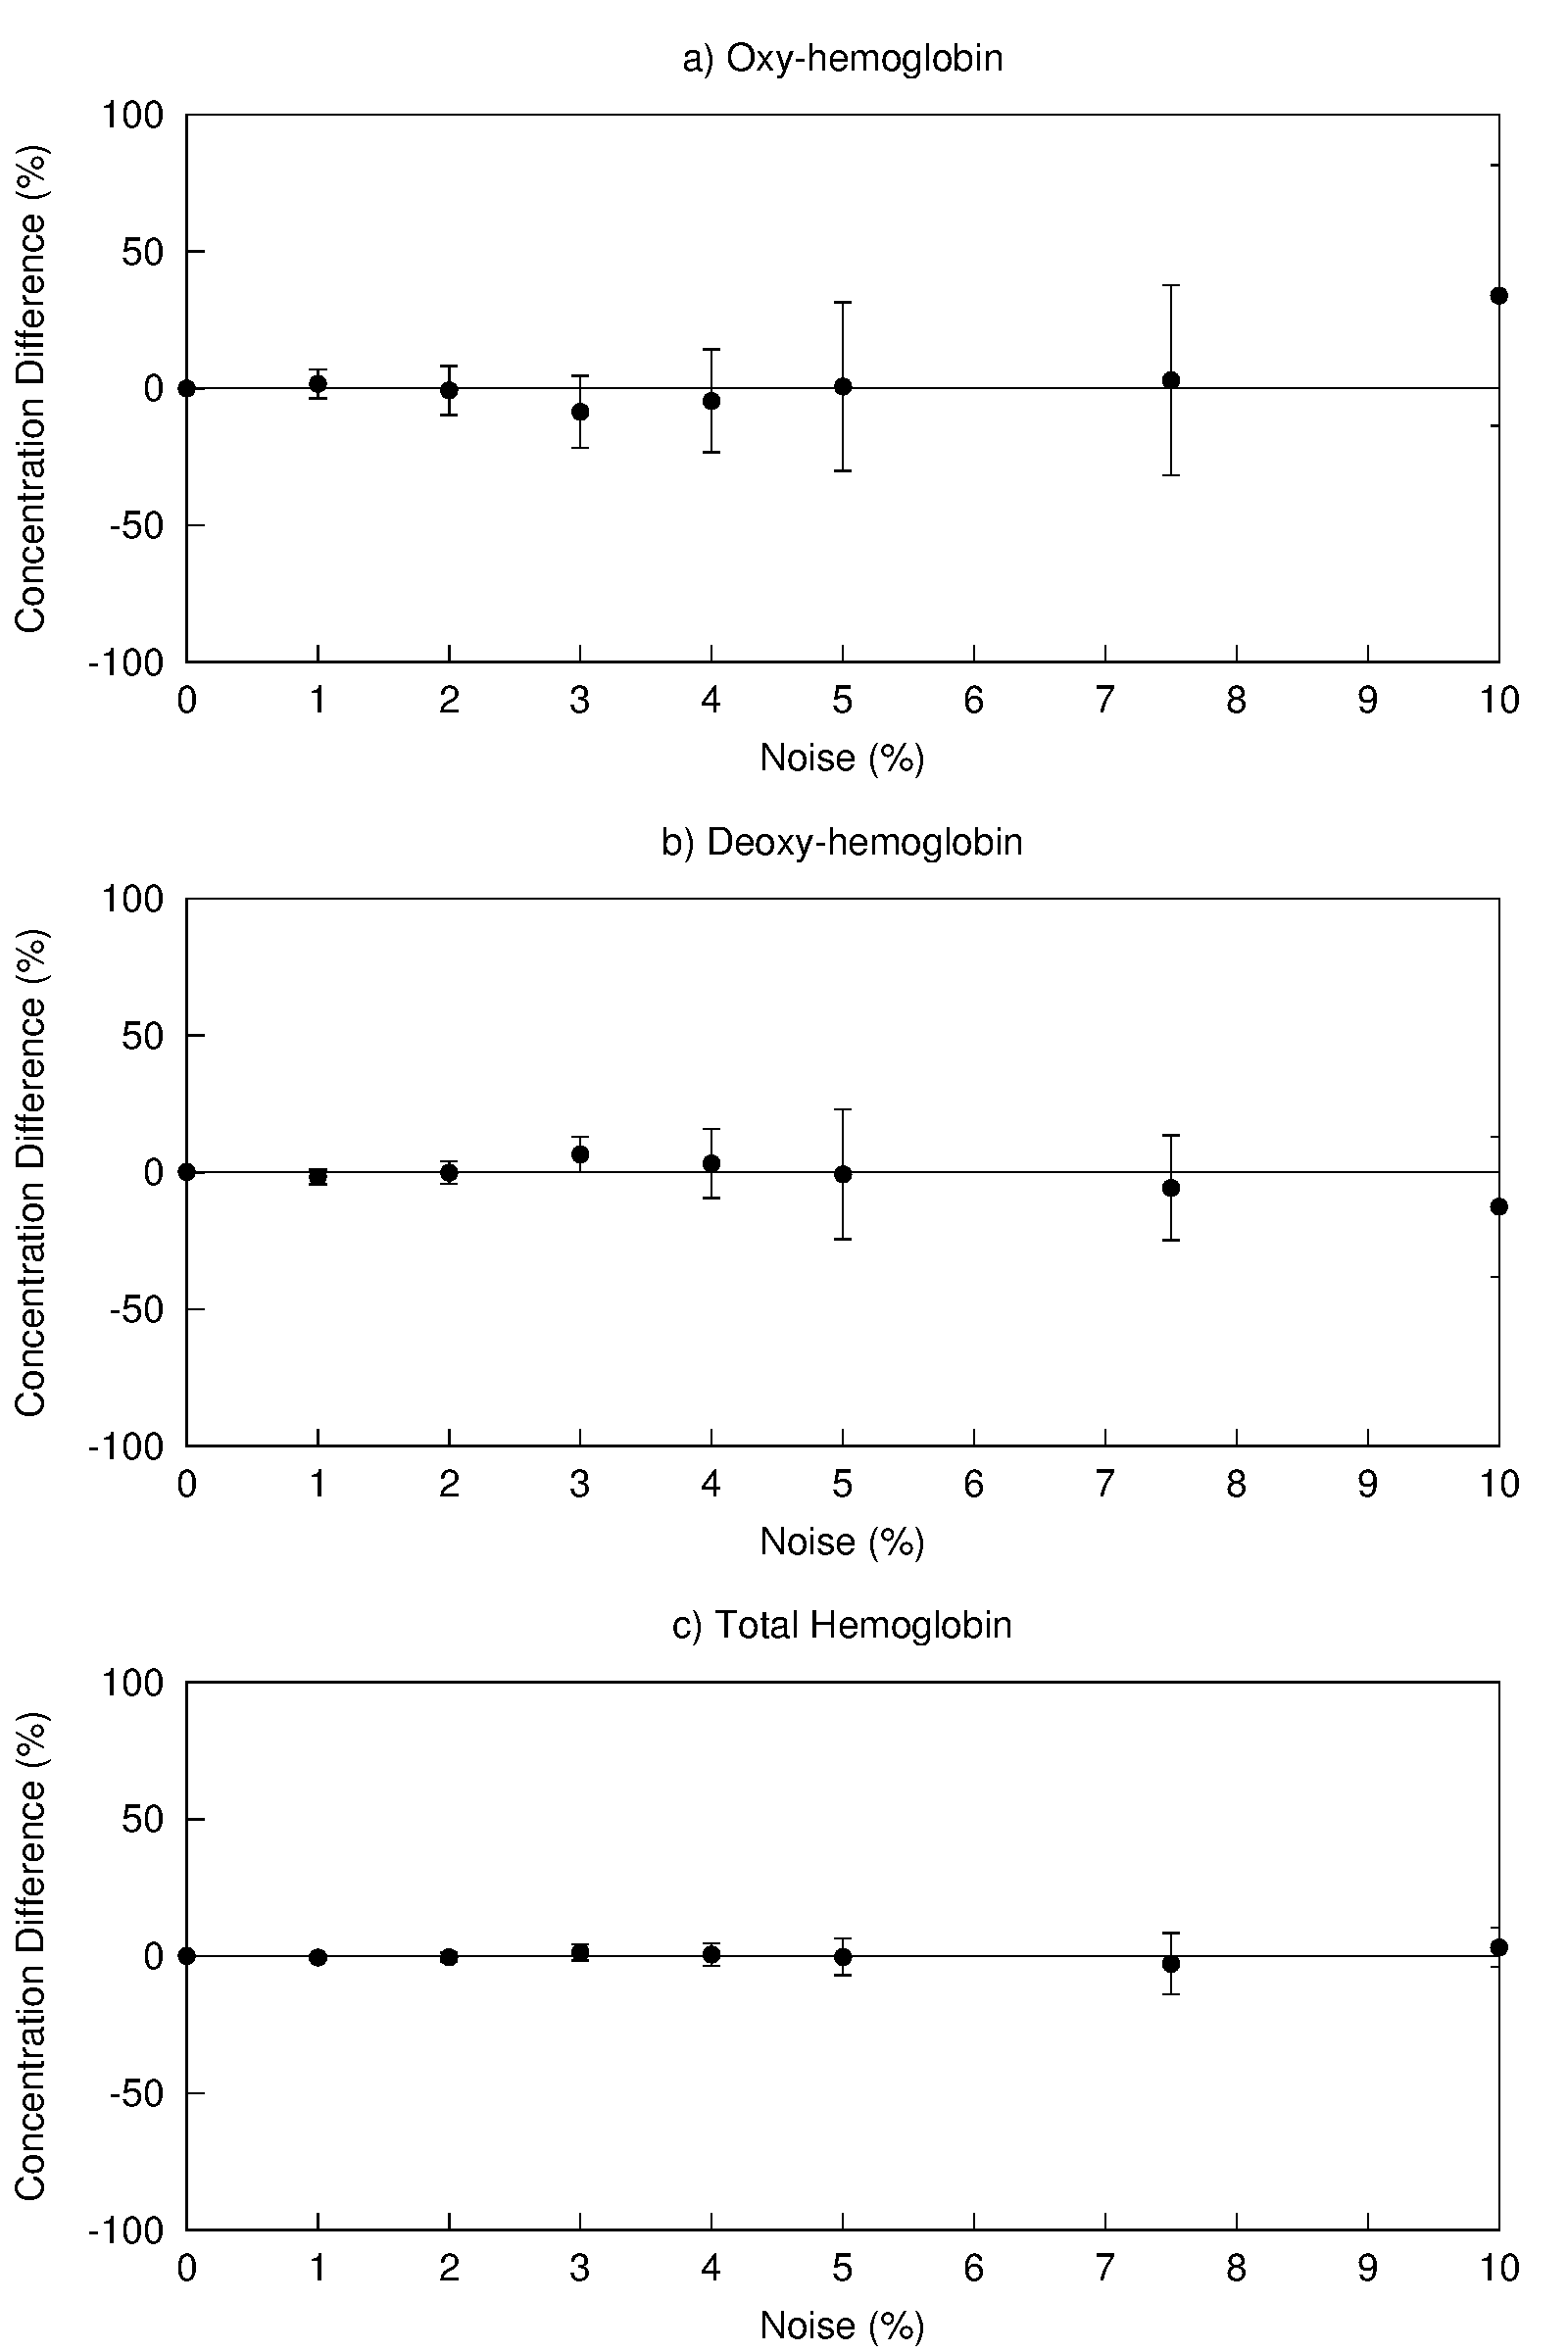
\includegraphics[width=0.8\textwidth]{figures/p3-oxy_deoxy_total.png}
	\caption[Percent differences between the recovered and input hemoglobin concentrations]{\label{fig:p3-oxy_deoxy_total}Percent differences between the recovered and input concentrations for a) oxy-hemoglobin and b) deoxy-hemoglobin. When combined into a total hemoglobin concentration (c), the standard deviation (represented by error bars) is consistently reduced.}
\end{figure}

The results are the same for the Type V reflectance spectra, which suggests that melanin, a broad spectrum absorber, does not mask the absorption effects of hemoglobin within the wavelength range of interest.

Further inspection of Figure~\ref{fig:p3-oxy_deoxy_total}c indicates that the noise generally increases the uncertainty for single measurements. This is expected, since the hemoglobin spectral features become harder to differentiate as the noise increases, particularly for higher melanin and/or lower hemoglobin concentrations. For the noise levels associated with the IS system (two percent), the difference between the input and recovered total hemoglobin concentrations did not exceed five percent for any of the 240 individual test spectra processed. Since this level of variation is of the same order as the observed daily variation in hemoglobin concentration,\cite{Fullerton1996} it is considered acceptable.

\subsubsection{Effect of an Incorrect Scatter Coefficient Spectrum}
The eight Fitzpatrick Type III reflectance spectra with increasing total hemoglobin concentrations and characteristic noise were processed using the model and different assumed reduced scattering coefficient spectra. The maximum percent difference between the recovered and input total hemoglobin concentrations increased linearly with the reduced scattering coefficient spectrum (not shown). For example, if the model employed an assumed reduced scattering coefficient spectrum that was ten percent higher than the actual input scatter coefficient spectrum, the recovered total hemoglobin concentration also had a maximum difference on the order of ten percent. This agrees with what is known about the coupled nature of the scattering and absorption coefficients: that if both of the coefficients are increased by the same factor, they produce the same total diffuse reflectance.

There is a large body of research regarding the reduced scattering coefficient spectrum of skin and therefore, it is unlikely that the assumed reduced scatter spectrum will ever exceed an absolute difference of ten percent unless the individual suffers from a condition that causes abnormal keratin or collagen fiber growth. As such, it is expected that the total hemoglobin concentration for most individuals can be recovered to within ten percent.

The diffuse reflectance model assumed a homogeneous single layer, while skin is actually a layered structure with melanin in the epidermal layer and hemoglobin in the dermal layer. Consequently, only the recovery of a perceived or apparent chromophore concentration is possible with the model. The recovered total hemoglobin concentrations expressed as a percent increase relative to an initial, baseline measurement can act as a proxy measure of the actual hemoglobin concentration found in the dermal layer. It also has the added benefit of removing any effects caused by an incorrectly assumed reduced scattering coefficient, as shown in Figure~\ref{fig:p3-incorrect_scatter}. When expressed in this manner, the percent difference only exceeds five percent for atypical skin conditions such as when the hemoglobin concentration is alarmingly low (25 percent) or when the assumed reduced scattering coefficient deviates from average values by greater than 50 percent.

\begin{figure}
	\centering 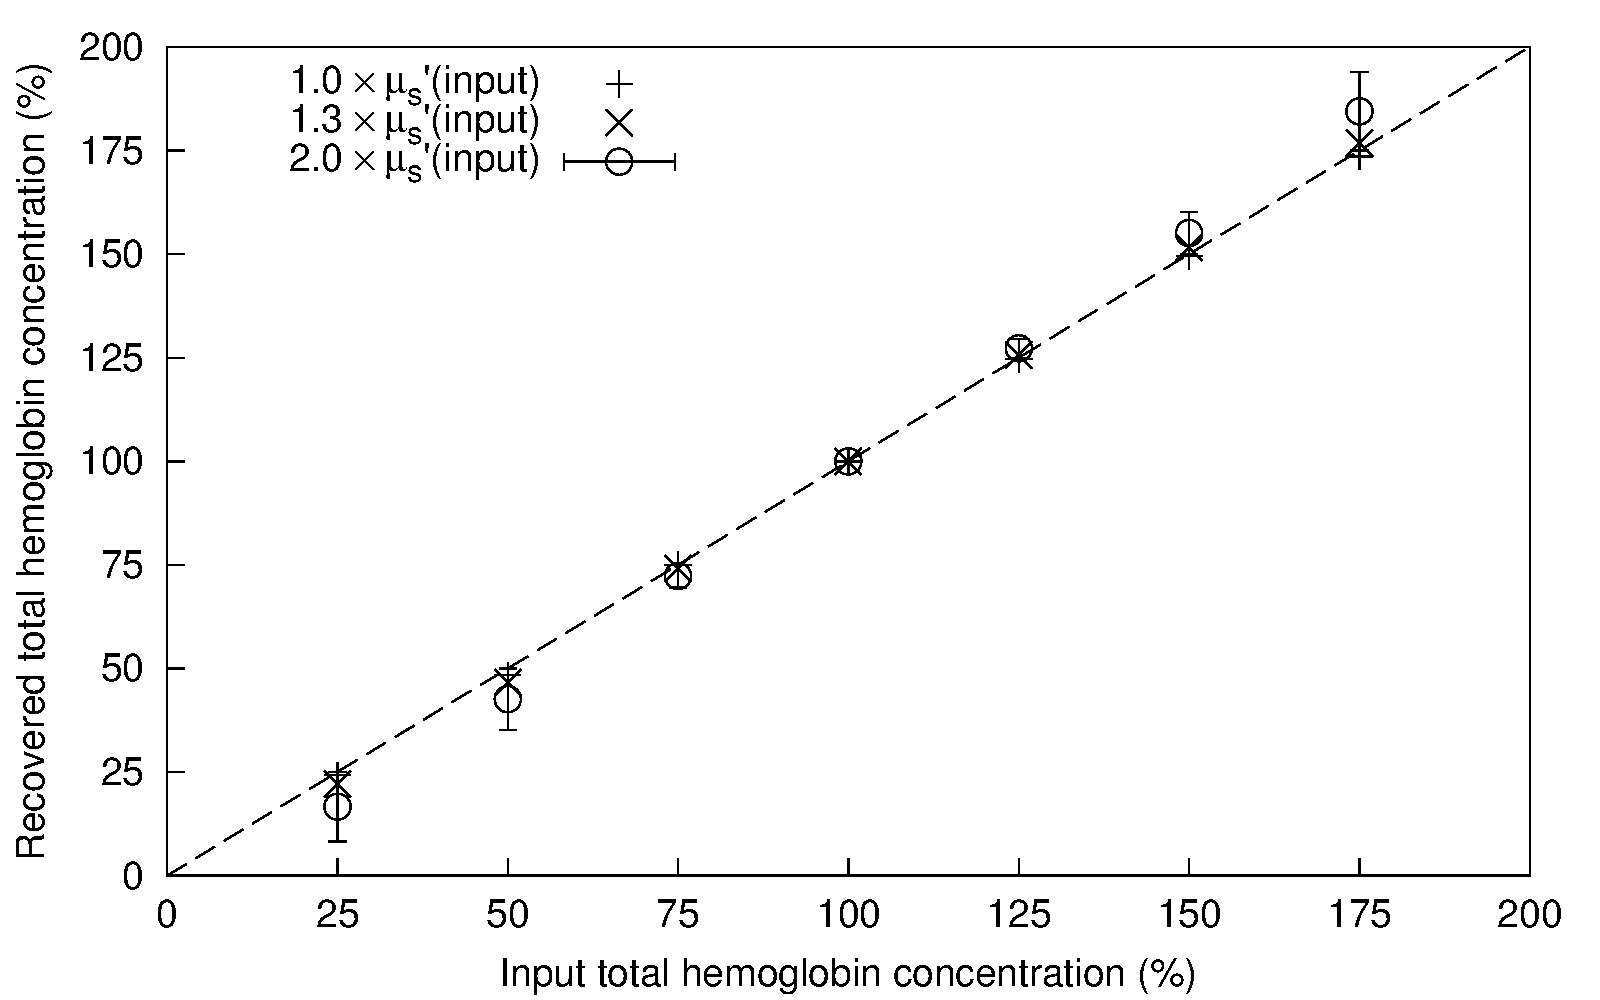
\includegraphics[width=0.8\textwidth]{figures/p3-incorrect_scatter.png}
	\caption[Total hemoglobin concentration recovered with the erroneous reduced scattering coefficients]{\label{fig:p3-incorrect_scatter}Total hemoglobin concentration recovered with the erroneous reduced scattering coefficients ($\mu_s'$) as a function of input total hemoglobin concentration. When the hemoglobin concentration is expressed as a fraction of a baseline measurement, the effects of an incorrectly assumed reduced scatter coefficient spectrum are removed. The line of unity has been added for visualization purposes. Error bars are only shown for the $2.0 \times \mu_s'$ data series.}
\end{figure}

\subsubsection{Effect of Changes to Background Absorption}
\label{sec:effect_bkg}
The relative total hemoglobin concentrations were recovered from the Fitzpatrick Type III reflectance spectra containing simultaneously increasing hemoglobin and background absorber concentrations (including melanin) using the model. In order to compare the performance of the model with common LIR techniques, the Dawson corrected Erythema Index\cite{Dawson1980} (EI\textsubscript{c}) was also calculated. The Dawson model was chosen because it was one of the first models created and is commonly cited in the literature. The total hemoglobin concentrations, expressed as a percent increase from the baseline measurement, are shown in Figure~\ref{fig:p3-bkg_changes} for both approaches.

\begin{figure}
	\centering 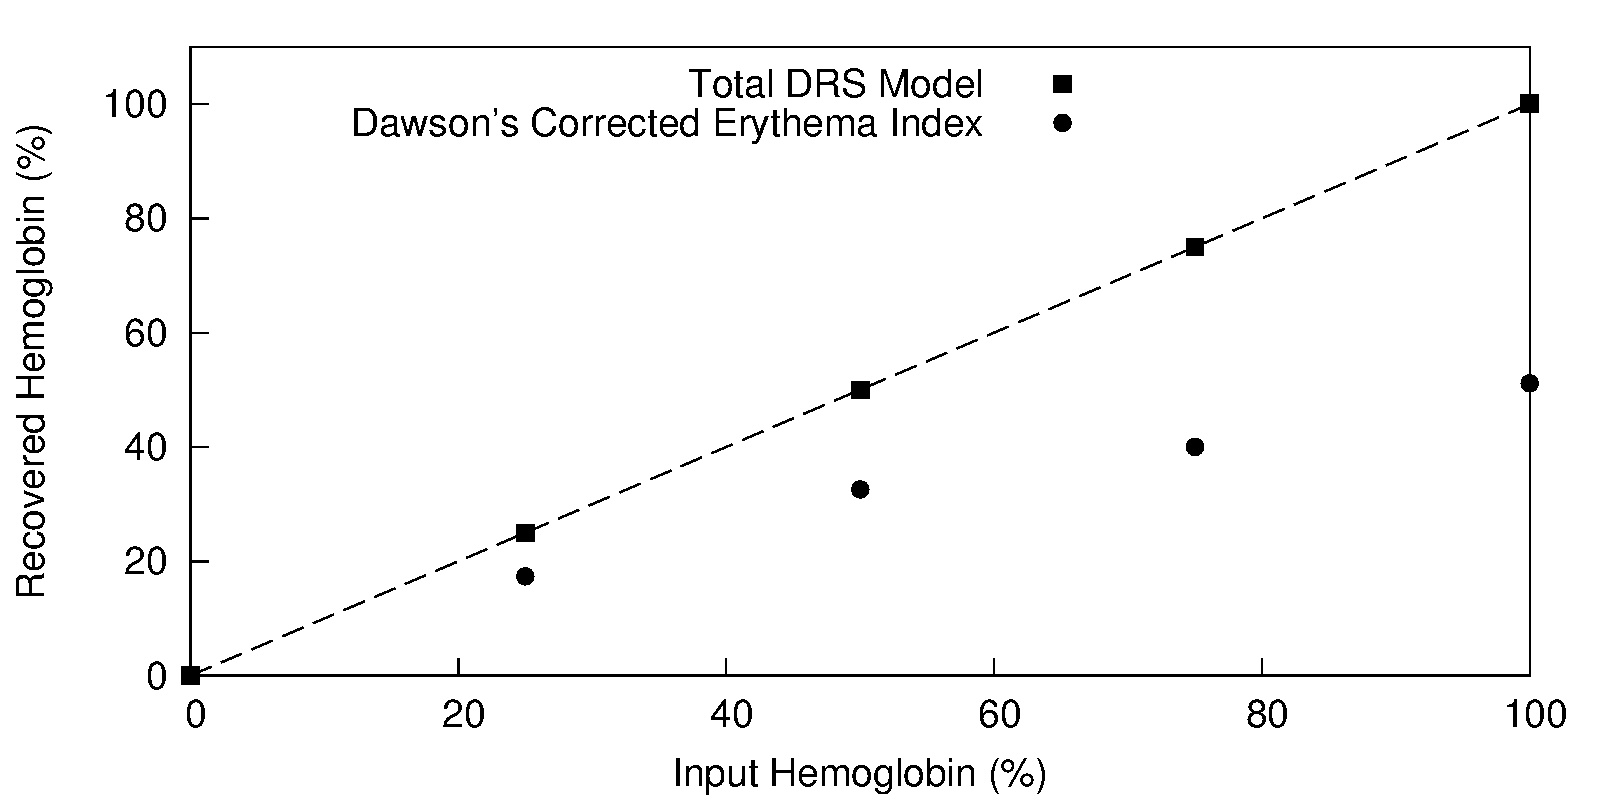
\includegraphics[width=0.8\textwidth]{figures/p3-bkg_changes.png}
	\caption[Hemoglobin recovery with changing background absorber concentrations]{\label{fig:p3-bkg_changes}Percent increases in the total hemoglobin for reflectance spectra with simultaneously increasing hemoglobin and background absorbers. The model was able to account for changes in the background absorption and follows the line of unity, while the Dawson approach underestimates the increase in hemoglobin concentration.}
\end{figure}

Increases in the background absorption were found to have no impact on the relative total hemoglobin concentrations recovered with the model, as it was able to adjust the background absorption parameters to account for these changes. However, since the EI\textsubscript{c} equates relative hemoglobin changes to a change in the area under the LIR curve, the decrease in area due to the increased background absorption is erroneously interpreted, resulting in an under-estimation of the relative total hemoglobin.

\subsection{Empirical Determination of the Scattering Losses Correction Factor}
Consideration of the SLCFs from the MC simulations (Section~\ref{sec:SLCF_methods}) as a function of the absorption and reduced scattering coefficients indicated that there were two distinct regions within the data that roughly corresponded to values for which the diffusion approximation was valid, and for which the diffusion approximation did not hold. Inspection of the boundaries of the diffusion theory region suggested that it was approximately limited to values where the absorption coefficient was less than or equal to 5 percent of the reduced scattering coefficient. This agrees with the generally accepted limit on the diffusion theory which states that the absorption coefficient should be less than 10 percent of the reduced scattering coefficient. Since the model and the prediction of the SLCF both depend on diffusion theory, only those points in the calculated reflectance spectra (and their corresponding points in the measured spectra) that meet the optical property criterion of diffusion theory may be used in the fitting algorithm. SLCFs within the diffusion theory region ranged from 0.5 to 1.0 while values outside of the diffusion theory region exceeded 1.0, which could only be possible if additional light was being scattered into the IS. Only points where the relationship between the absorption and reduced scattering coefficient satisfied the diffusion theory were used to determine the functional form of the SLCF.

Scatter plots of the SLCF as a function of the absorption coefficient for single values of the reduced scattering coefficient (iso-lines) indicated a linear relationship with respect to the natural logarithm of the absorption coefficient. The scaling coefficient has a power-law relationship with the reduced scattering coefficient, resulting in a function form of,

\begin{equation}
\label{eq:SLCF}
	SLCF(\mu_a,\mu_s') = a \times \mu_s'^b \ln(\mu_a) + c
\end{equation}

The Intralipid\textregistered~phantom measurements were used to confirm Equation~\ref{eq:SLCF}, with triplets outside of the diffusion theory region omitted. This empirical fit was used to correct for scattering losses in the \emph{in vivo} study analysis.

\subsection{\emph{In Vivo} Study Analysis}
Each IS measurement from the \emph{in vivo} study was processed with the model and fitting algorithm as well as with the Dawson model for comparison purposes. A complete report of the analysis of the Dawson model was performed by McKee et al. (2013).\cite{McKee2013} A sample fit of the total DRS model to an individual IS measurement is shown in Figure~\ref{fig:p3-sample_fit}. Measured spectra with greater hemoglobin concentrations were observed to yield better fits with the model within the 520-580 nm region. This may be attributed to the difficulty of, and ambiguity in, combining the available extinction coefficient spectra in the absence of distinct hemoglobin spectral features. 

\begin{figure}
	\centering 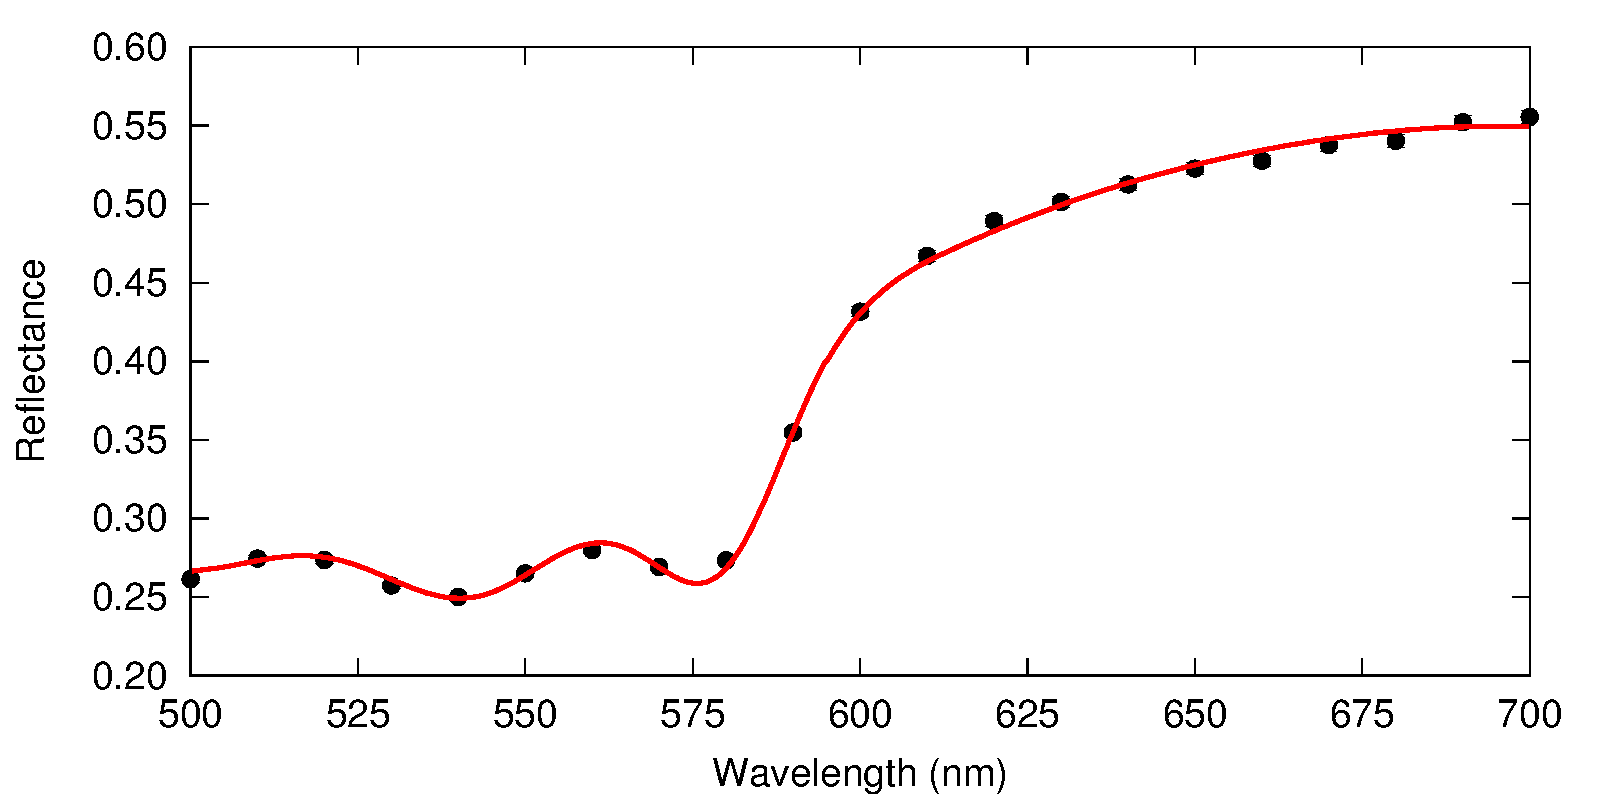
\includegraphics[width=0.8\textwidth]{figures/p3-sample_fit.png}
	\caption[Sample DRS spectrum and model fit]{\label{fig:p3-sample_fit}Sample spectrum ($\bullet$) and fit (red line). The measured spectrum has been down-sampled for illustration purposes. Measurement error bars are too small to be visible.}
\end{figure}

Based on the observations from Section~\ref{sec:model_char} that: (1) it is difficult to separate the oxy- and deoxy-hemoglobin contributions, and (2) that a relative increase in hemoglobin concentration removes any effects due to an incorrectly assumed reduced scattering coefficient spectrum, both the total hemoglobin concentration and corrected erythema index were expressed as a percent increase from the average of the baseline measurements. A sample time series of one of the volunteers is shown in Figure~\ref{fig:p3-lido_epi}.

\begin{figure}
	\centering 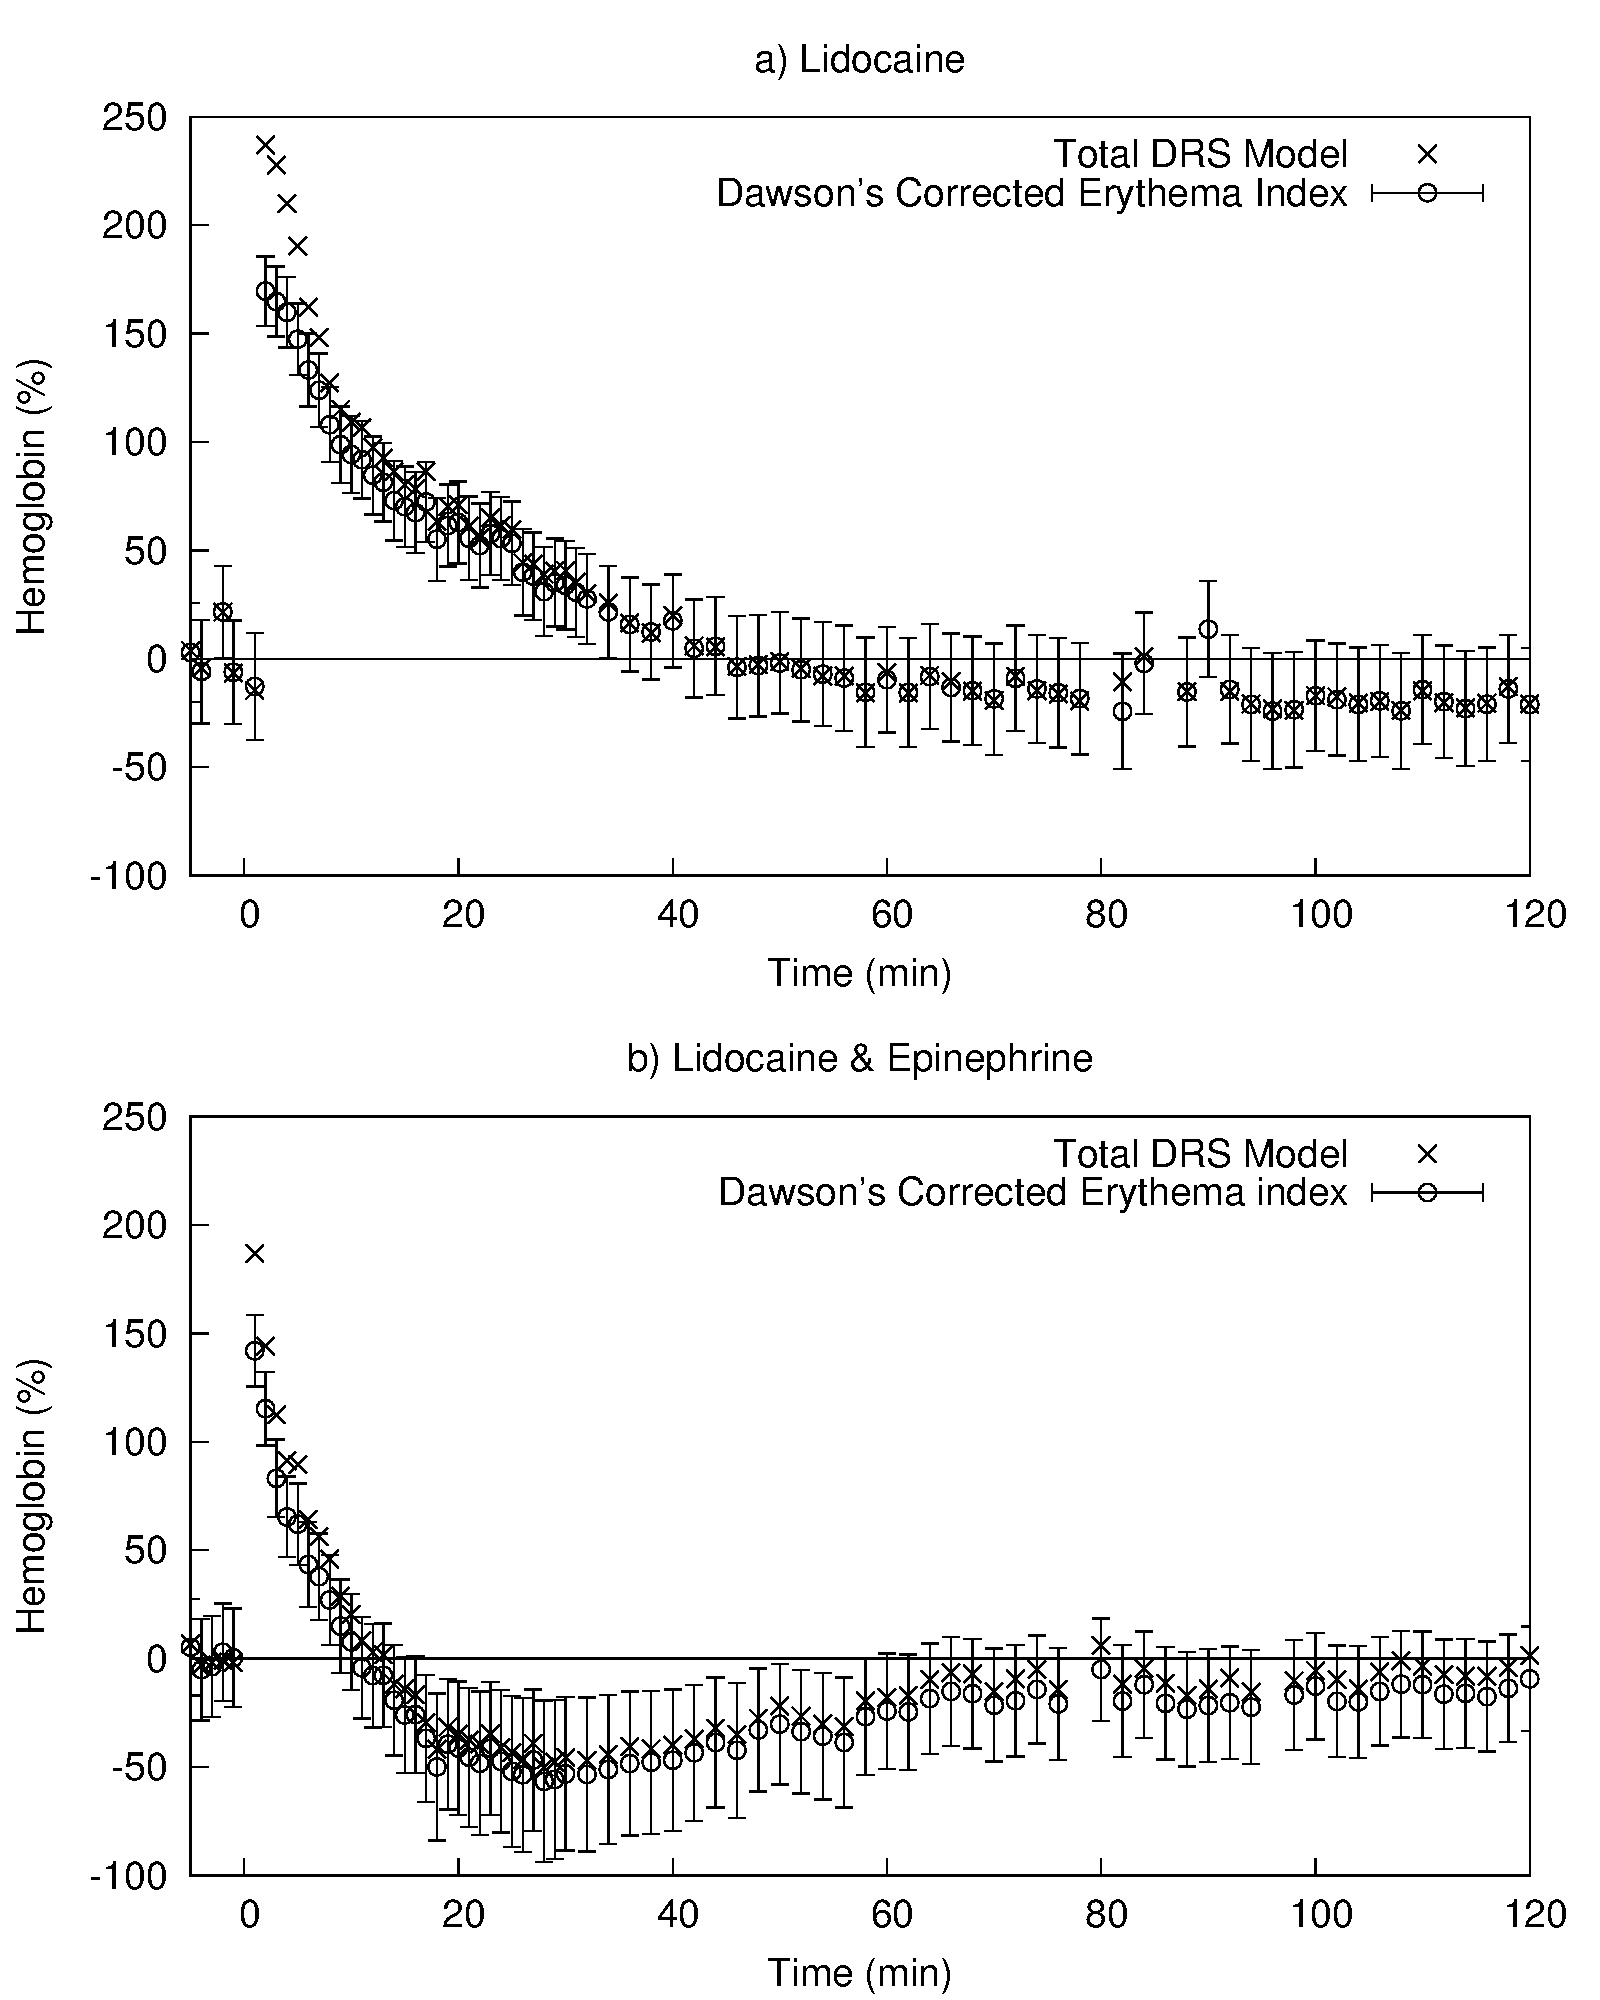
\includegraphics[width=0.8\textwidth]{figures/p3-lido_epi.png}
	\caption[Hover and figure index text]{\label{fig:p3-lido_epi}Sample time series for a single volunteer using both the total DRS model and the Dawson EI model. Error bars are shown only for the Dawson model as the returned standard deviation for the total DRS model is consistently less than 2 percent and not visible on this scale.}
\end{figure}

The two methods agree everywhere except immediately following the injection. This difference may be due to initial bleeding and/or swelling following the insertion of the needle, which would have led to changes in the scattering and/or the relative concentrations of the chromophores from the baseline measurements. Since the LIR approach was shown in Section~\ref{sec:effect_bkg} to be unable to correctly interpret changes to non-hemoglobin chromophore concentrations, it is most likely that the erythema index is underestimating the skin redness in this situation.

\section{Conclusion}
In this paper, a model was derived for the total diffuse reflectance spectrum based on a semi-infinite, broad beam homogeneous geometry. The model was then used to interpret total diffuse reflectance spectra obtained with an integrating sphere placed on the skin, following corrections for the perturbations associated with this measurement technique. Characterization of the model and system showed that this approach was insensitive to characteristic noise, and able to account for any deviations from the assumed reduced scattering coefficient spectrum. When compared to a common log inverse reflectance approach, the model proved superior in its ability to successfully interpreted changes to background absorber concentrations. Finally, the model was applied to reflectance spectra obtained during an in vivo study and compared to analysis using the Dawson erythema index. The two methods agreed over the majority of the measurement period, but differed immediately following injection, most likely due to the Dawson model incorrectly interpreting the acute response to the needle insertion.

\section*{Acknowledgments}
The authors would like to thank Dr. Daniel E. McKee for his help with the in vivo study and Dr. Gabriel A. Devenyi for his help with the Monte Carlo simulations. Monte Carlo simulations were performed using the facilities at SHARCNET (Shared Hierarchical Research Computing Network: \url{www.sharcnet.ca}) and Compute/Calcul Canada. This work was financially supported by the Natural Sciences and Engineering Research Council of Canada (NSERC).